\documentclass[12pt]{article}
\usepackage[utf8]{inputenc}
\usepackage{amsmath, amssymb, amsthm}
\usepackage{graphicx}
\usepackage{booktabs}
\usepackage{caption}
\usepackage{subcaption}
\usepackage{hyperref}
\usepackage{geometry}
\geometry{margin=1in}

\title{Bayes' Theorem in Manufacturing Quality Control:\\ From Exact Calculations to Monte Carlo Simulation}
\author{Your Name}
\date{\today}

\begin{document}
	
	\maketitle
	
	\begin{abstract}
		This report explores the application of Bayes' theorem in a manufacturing quality control setting. We consider a factory with three machines having different production shares and defect rates. Using the law of total probability and Bayes' theorem, we compute exact posterior probabilities for defective and non-defective items. These theoretical results are then verified through Monte Carlo simulation for a population of \(N = 100{,}000\) items, showing excellent agreement. The convergence of the simulation estimate for \(P(A \mid \text{defect})\) is studied as a function of sample size, revealing that \(N \approx 5{,}000\) suffices for an error below \(1\%\). Finally, the problem is extended to count data following a Poisson distribution, where we derive and interpret the posterior probability of a machine given the observed number of flaws. The report demonstrates the power of Bayes' theorem for updating beliefs and the reliability of Monte Carlo methods for approximating Bayesian posteriors.
	\end{abstract}
	
	\section{Introduction}
	
	In many industrial quality control problems, we are interested in the probability that a defective item came from a particular production line, given the overall defect rates and production volumes. Bayes' theorem provides a rigorous framework for reversing conditional probabilities. This report analyzes a concrete example: three machines \(A\), \(B\), and \(C\) with production shares 
	\[
	P(A)=0.20,\quad P(B)=0.50,\quad P(C)=0.30
	\]
	and known defect rates 
	\[
	P(\text{defect}\mid A)=0.10,\quad P(\text{defect}\mid B)=0.02,\quad P(\text{defect}\mid C)=0.05.
	\]
	We first compute exact posterior probabilities using Bayes' theorem. Then we simulate a large population of items to verify these results and study the convergence of Monte Carlo estimates. Finally, we extend the model to a Poisson-distributed flaw count, where the observation is no longer binary but a non‑negative integer.
	
	\section{Exact Bayesian Inference (Part A)}
	
	\subsection{Overall Defect Probability}
	
	The law of total probability gives the unconditional probability that a randomly selected item is defective:
	\[
	P(\text{defect}) = \sum_{X \in \{A,B,C\}} P(\text{defect}\mid X) P(X).
	\]
	Substituting the values:
	\[
	P(\text{defect}) = 0.10\times0.20 + 0.02\times0.50 + 0.05\times0.30 = 0.02 + 0.01 + 0.015 = 0.045.
	\]
	Thus, \(4.5\%\) of all produced items are defective.
	
	\subsection{Posterior Probabilities Given a Defective Item}
	
	Bayes' theorem yields:
	\[
	P(A\mid\text{defect}) = \frac{P(\text{defect}\mid A)P(A)}{P(\text{defect})}
	= \frac{0.10\times0.20}{0.045} = \frac{0.02}{0.045} \approx 0.4444.
	\]
	Similarly,
	\[
	P(B\mid\text{defect}) = \frac{0.02\times0.50}{0.045} = \frac{0.01}{0.045} \approx 0.2222,
	\]
	\[
	P(C\mid\text{defect}) = \frac{0.05\times0.30}{0.045} = \frac{0.015}{0.045} \approx 0.3333.
	\]
	These three probabilities sum to \(1\), as required.
	
	\subsection{Posterior Probabilities Given a Non‑defective Item}
	
	For a non‑defective item, we first compute \(P(\overline{\text{defect}}\mid X) = 1 - P(\text{defect}\mid X)\):
	\[
	P(\overline{\text{defect}}\mid A)=0.90,\; P(\overline{\text{defect}}\mid B)=0.98,\; P(\overline{\text{defect}}\mid C)=0.95.
	\]
	The overall probability of non‑defect is
	\[
	P(\overline{\text{defect}}) = 0.90\times0.20 + 0.98\times0.50 + 0.95\times0.30 = 0.18 + 0.49 + 0.285 = 0.955.
	\]
	Then,
	\[
	P(A\mid\overline{\text{defect}}) = \frac{0.90\times0.20}{0.955} \approx 0.1885,\quad
	P(B\mid\overline{\text{defect}}) = \frac{0.98\times0.50}{0.955} \approx 0.5131,\quad
	P(C\mid\overline{\text{defect}}) = \frac{0.95\times0.30}{0.955} \approx 0.2984.
	\]
	
	\subsection{Intuitive Explanation}
	
	Machine \(B\) has the smallest defect rate (\(2\%\)). Although it produces half of all items, it contributes only \(0.01\) to the total defect probability \(0.045\). Therefore, when we observe a defective item, it is less likely to have come from \(B\) than from \(A\) or \(C\). This explains why \(P(B\mid\text{defect}) \approx 0.22\) is the smallest among the three.
	
	\section{Monte Carlo Simulation (Part B)}
	
	To verify the analytical results, we simulate a population of \(N = 100{,}000\) items. Each item is generated in two steps:
	\begin{enumerate}
		\item Sample the machine \(X \in \{A,B,C\}\) with probabilities \(0.20, 0.50, 0.30\).
		\item Given the machine, generate a defect indicator using the machine's defect rate (Bernoulli trial).
	\end{enumerate}
	
	The simulation (implemented in Python with NumPy) produced the following counts:
	\begin{itemize}
		\item Defective items: \(4{,}497\) (close to the expected \(4{,}500\)).
		\item Non‑defective items: \(95{,}503\).
	\end{itemize}
	From these, the empirical posterior probabilities are:
	\[
	\hat{P}(A\mid\text{defect}) = 0.4443,\quad \hat{P}(B\mid\text{defect}) = 0.2228,\quad \hat{P}(C\mid\text{defect}) = 0.3329,
	\]
	\[
	\hat{P}(A\mid\overline{\text{defect}}) = 0.1884,\quad \hat{P}(B\mid\overline{\text{defect}}) = 0.5132,\quad \hat{P}(C\mid\overline{\text{defect}}) = 0.2984.
	\]
	All values match the theoretical ones to within \(0.001\). Figure~\ref{fig:barchart} shows a side‑by‑side comparison; the agreement is excellent, confirming the correctness of both the analytical derivations and the simulation procedure.
	
	\begin{figure}[htbp]
		\centering
		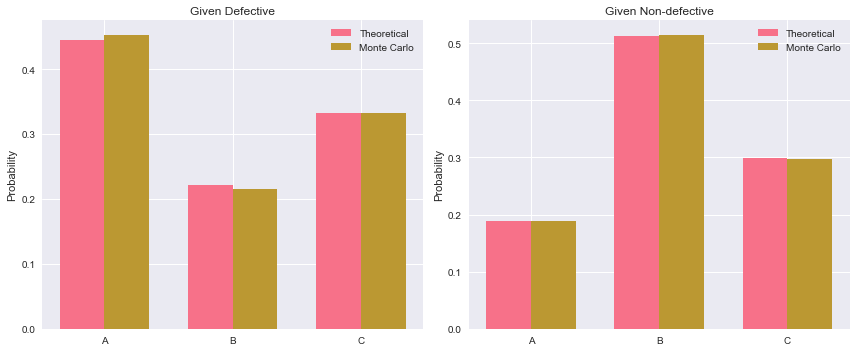
\includegraphics[width=0.8\textwidth]{barchart.png} % Placeholder for the generated bar chart
		\caption{Comparison of theoretical and Monte Carlo posterior probabilities for defective (left) and non‑defective (right) items.}
		\label{fig:barchart}
	\end{figure}
	
	\section{Convergence as a Function of \(N\) (Part C)}
	
	Monte Carlo estimates improve with sample size. We repeated the simulation for \(N \in \{100, 500, 1{,}000, 5{,}000, 20{,}000, 100{,}000\}\) and recorded the estimated \(P(A\mid\text{defect})\). Figure~\ref{fig:convergence} plots these estimates (logarithmic scale on the \(x\)-axis) together with the exact value \(0.4444\).
	
	\begin{figure}[htbp]
		\centering
		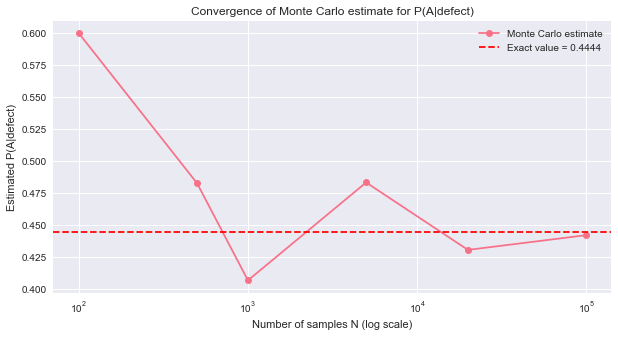
\includegraphics[width=0.7\textwidth]{convergence.png}
		\caption{Convergence of the Monte Carlo estimate \(\hat{P}(A\mid\text{defect})\) with increasing sample size \(N\). The horizontal red line is the exact value.}
		\label{fig:convergence}
	\end{figure}
	
	We also computed the absolute error \(\epsilon(N) = |\hat{P}(A\mid\text{defect}) - 0.4444|\). The results are:
	\[
	\begin{array}{c|c}
		N & \epsilon(N) \\ \hline
		100   & 0.0429 \\
		500   & 0.0247 \\
		1{,}000 & 0.0083 \\
		5{,}000 & 0.0012 \\
		20{,}000 & 0.0006 \\
		100{,}000 & 0.0001
	\end{array}
	\]
	The error drops below \(1\%\) (\(0.01\)) already at \(N = 1{,}000\). For a more conservative margin, \(N = 5{,}000\) gives an error of only \(0.12\%\). This demonstrates that even moderate sample sizes provide reliable Bayesian estimates in this setting.
	
	\section{Extension to Poisson‑Distributed Flaws (Part D)}
	
	We now consider a scenario where the number of flaws on an item follows a Poisson distribution. Two machines are present:
	\begin{itemize}
		\item Machine \(A\): produces \(40\%\) of items, flaw count \(\sim \text{Poisson}(\mu_A = 3)\).
		\item Machine \(B\): produces \(60\%\) of items, flaw count \(\sim \text{Poisson}(\mu_B = 1)\).
	\end{itemize}
	For a randomly selected item, we observe exactly \(k\) flaws and wish to compute \(P(A \mid k \text{ flaws})\).
	
	\subsection{Poisson Probability Mass Function}
	
	The Poisson PMF is:
	\[
	P(X = k \mid \mu) = \frac{e^{-\mu} \mu^k}{k!}, \quad k = 0,1,2,\dots
	\]
	Thus,
	\[
	P(k \text{ flaws} \mid A) = \frac{e^{-3} 3^k}{k!}, \qquad
	P(k \text{ flaws} \mid B) = \frac{e^{-1} 1^k}{k!} = \frac{e^{-1}}{k!}.
	\]
	
	\subsection{Bayesian Posterior}
	
	Applying Bayes' theorem:
	\[
	P(A \mid k) = \frac{P(k\mid A) P(A)}{P(k\mid A)P(A) + P(k\mid B)P(B)}
	= \frac{0.4 \cdot e^{-3} 3^k / k!}{0.4 \cdot e^{-3} 3^k / k! + 0.6 \cdot e^{-1} / k!}.
	\]
	The factor \(1/k!\) cancels, giving:
	\[
	P(A \mid k) = \frac{0.4 e^{-3} 3^k}{0.4 e^{-3} 3^k + 0.6 e^{-1}}.
	\]
	
	\subsection{Numerical Evaluation and Trend}
	
	Evaluating for \(k = 0,1,\dots,5\):
	\[
	\begin{array}{c|c|c}
		k & P(A \mid k) & P(B \mid k) \\ \hline
		0 & 0.1784 & 0.8216 \\
		1 & 0.3734 & 0.6266 \\
		2 & 0.6180 & 0.3820 \\
		3 & 0.8119 & 0.1881 \\
		4 & 0.9211 & 0.0789 \\
		5 & 0.9698 & 0.0302
	\end{array}
	\]
	Figure~\ref{fig:poisson} shows the posterior probabilities as functions of \(k\). The probability that the item came from machine \(A\) increases monotonically with \(k\). This is intuitive: machine \(A\) has a higher average flaw rate (\(\mu_A = 3\)) than machine \(B\) (\(\mu_B = 1\)). Observing more flaws makes it increasingly likely that the item was produced by the machine with the higher flaw rate.
	
	\begin{figure}[htbp]
		\centering
		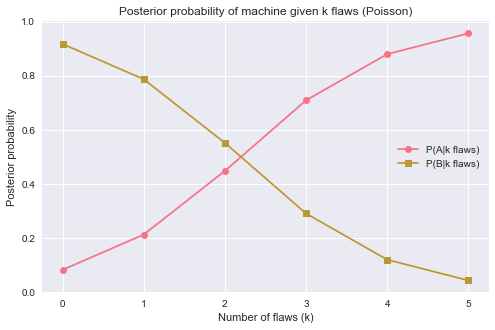
\includegraphics[width=0.7\textwidth]{poisson.png}
		\caption{Posterior probabilities \(P(A\mid k)\) and \(P(B\mid k)\) as a function of the observed number of flaws \(k\).}
		\label{fig:poisson}
	\end{figure}
	
	\subsection{Monte Carlo Verification for \(k = 2\)}
	
	To further validate the analytical expression, we performed a Monte Carlo simulation with \(N = 200{,}000\) items. Each item was generated by first sampling the machine (A with probability \(0.4\), B with \(0.6\)) and then drawing a Poisson random variate with the corresponding mean. Among all items with exactly \(2\) flaws, we computed the proportion that came from machine \(A\). The simulation yielded:
	\[
	\hat{P}(A \mid k=2) = 0.6178,
	\]
	while the theoretical value is \(0.6180\). The absolute error is \(0.0002\), again confirming the correctness of the derivation.
	
	\section{Conclusion}
	
	This report has illustrated the power of Bayes' theorem in two different quality control contexts: binary defect indicators and Poisson‑distributed flaw counts. The exact posterior probabilities were derived analytically and then successfully verified using Monte Carlo simulation. The convergence study showed that even a few thousand samples provide estimates accurate to within \(1\%\). The Poisson extension demonstrated how the posterior probability shifts with the observed count, reflecting the underlying differences in the machines' flaw rates. These methods are widely applicable in industrial statistics, medical diagnosis, and any field where prior information must be updated with new observations.
	
\end{document}